\section{Structure of SU2}

\begin{frame}{Conservative Equations}
\begin{equation}
\frac{\partial \boldsymbol{U}}{\partial t}+\underbrace{\nabla \cdot \boldsymbol{F}^{c}}_{\text CONV\ TERM}-\overbrace{\nabla \cdot\left(\mu^{v k} \boldsymbol{F}^{v k}\right)}^{\text VISC\ TERM}=\boldsymbol{Q} \quad \text { in }\Omega,  \quad t>0
\end{equation}

Most SU2 scripts are located in the \textit{SU2\_CFD} and \textit{Common} folder, other folders contain very limited amount of codes concerning adaptive mesh, dual grid and \textit{e.t.c.} 

\begin{itemize}
    \item OS: Cross-platform
    \item Lang: C++, Python
    \item Mainly vertex-based dual mesh FVM, also supports FEM and primal grid
\end{itemize}
\end{frame}

\begin{frame}{Vertex-based Dual Grid}
\begin{figure}
    \centering
    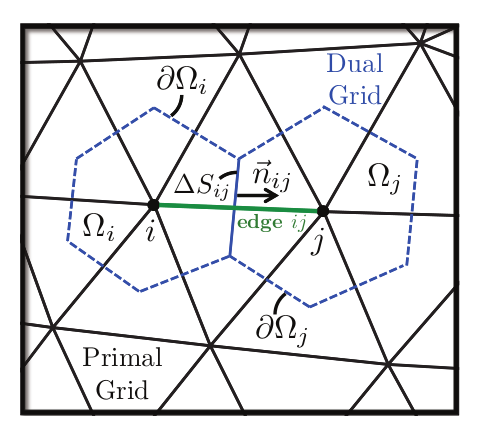
\includegraphics[width=0.5\linewidth]{figures/DualMeshControlVolume.png}
    \caption{Dual mesh control volumes surrounding two nodes, $i$ and $j$, in the domain interior.}
    % \label{fig:my_label}
\end{figure}


By virtue of the functionality of geometry-relevant source, researchers do not need to implement the area calculation step and are capable to use the face area and normal vector directly.

\end{frame}

\begin{frame}{CDriver}
CDriver controls instantiating and deleting major classes, just like a housekeeper.\\
\textbf{CDriver::StartSolver} loops over all external iterations to do the following pipeline
\begin{itemize}
    \item PreprocessExtIter
    \item DynamicMeshUpdate (optional)
    \item Run (SIngle ExtIteration)
    \item Update
    \item Monitor
    \item Output
\end{itemize}
\end{frame}

\begin{frame}{CDriver::Run }
CDriver::StartSolver method runs \emph{ExtIter} times the aforementioned pipeline. For steady and unsteady simulation, the procedure is similar, \textbf{steady} solution tends to be stable in the end, while for the \textbf{unsteady} simulation every ExtIter loop means an certain period of physical time development. 
\begin{itemize}
    \item \textbf{Preprocess}\\
            iteration\_container[iZone][Inst\_0]$\longrightarrow$ Preprocess
    \item \textbf{Zone Interface}\\
            interpolator\_container[iZone][jZone]$\longrightarrow$ Set\_TransferCoeff
            Transfer\_Data(iZone, jZone)\\
    \item \textbf{Iterate}\\
            iteration\_container[iZone][Inst\_0]$\longrightarrow$ Iterate
    \item \textbf{Check Convergence}
\end{itemize}
What does the \textbf{Iteration::Iterate} method do?
\end{frame}

\begin{frame}{CIteration::Iterate}
The CIteration::Iterate loops over all the solver to iterate in all equations.
\begin{itemize}
    \item \textbf{Update Global Parameters}\\
    config[val\_iZone]$\longrightarrow$ setGlobalParams
    \item \textbf{Solve the Equation}\\
    integration[val\_iZone][val\_iInst]...\\
    ...[FLOW\_SOL]$\longrightarrow$MultiGrid\_Iteration\\
    ...[TURB\_SOL]$\longrightarrow$SingleGrid\_Iteration\\
    ...[TRAN\_SOL]$\longrightarrow$SingleGrid\_Iteration\\
    ...[HEAT\_SOL]$\longrightarrow$SingleGrid\_Iteration
    \item \textbf{Mesh Update}
    \item \textbf{Output}
    
\end{itemize}
Now our focus moves from \emph{CIteration} class to \emph{CIntegration} class.
\end{frame}

\begin{frame}{CIntegration::Iteration}
Most simple case is CIntegration::SingleGrid\_Iteration.

\begin{itemize}
    \item \textbf{Preprocessing}
    solver\_container[iZone][iInst][FinestMesh][SolContainer\_Position]\\$\longrightarrow$ Preprocessing\\$\longrightarrow$ Set\_OldSolution \\$\longrightarrow$ Set\_Timestep
    \item \textbf{Space Integration}
    Space\_Integration(...)
    \item \textbf{Time Integration}
    Time\_Integration(...)
    \item \textbf{Postprocessing}
\end{itemize}

The space integration will invoke \textbf{CSolver} class to compute the residual.
\end{frame}

\begin{frame}
\frametitle{CSolver}
One physical problem may consist of various equations.
CSolver controls its own conservative equation. 

e.g., RANS model in SU2 has three solvers working together, FLOW\_SOL, TURB\_SOL, TRAN\_SOL.



Let's have heat equation as an example.
Different spatial residual terms coexist in one equation.
\begin{itemize}
    \item \emph{CONV}, Convective terms caused by fluid motion.
    \item \emph{VISC}, Viscous terms caused by the gradient of temperature. 
\end{itemize}

\textbf{Space\_Integration}
solver\_container[MainSolver]...\\
\textbf{CONV\_TERM}$\longrightarrow$Centered\_Residual\quad$\longrightarrow$Upwind\_Residual\\
\textbf{VISC\_TERM}$\longrightarrow$Viscous\_Residual\\
\textbf{Source\_TERM}$\longrightarrow$Source\_Residual\\
\textbf{BC}$\longrightarrow$BC\_Euler\_wall(...)...\\
\textbf{Dual\_Time}$\longrightarrow$SetResidual\_DualTime

\end{frame}


\begin{frame}{CHeatSolver VISC TERM}
Apparently, the viscous term in heat equation means the temperature tends to be the same all over the domain.

For simple situation in solid material, the heat equation reads as
\begin{equation}
    \frac{\partial T}{\partial t} - \nabla\cdot(\alpha \nabla T) =0,
\end{equation}
where $\alpha$ is the thermal diffusivity and depends on whether the material is liquid or solid.

\begin{equation}
F_{ij}=\alpha \vec{S}\cdot \nabla T=\alpha \vec{S}\cdot \frac{T_j-T_I}{\left \| d_{ij} \right \|^2}\vec{d_{ij}}
\end{equation}
\begin{equation}
    \frac{\partial F_{ij}}{\partial T_i}=-\alpha \frac{\vec{S}\cdot \vec{d_{ij}}}{\left \| d_{ij} \right \|^2}
\end{equation}
BCs are similar, contributing residuals and Jacobian matrix to the overall LARGE SPARSE matrix.
\end{frame}


\lstset{keywordstyle=\color{red},keywords={court}}
\begin{lstlisting}
  eddy_viscosity_i = 0.0;
  eddy_viscosity_j = 0.0;
  laminar_viscosity = config->GetMu_ConstantND();
  Prandtl_Lam = config->GetPrandtl_Lam();
  Prandtl_Turb = config->GetPrandtl_Turb();

  for (iEdge = 0; iEdge < geometry->GetnEdge(); iEdge++) {

    iPoint = geometry->edge[iEdge]->GetNode(0);
    jPoint = geometry->edge[iEdge]->GetNode(1);

    /*--- Points coordinates, and normal vector ---*/

    numerics->SetCoord(geometry->node[iPoint]->GetCoord(),
                       geometry->node[jPoint]->GetCoord());
    numerics->SetNormal(geometry->edge[iEdge]->GetNormal());

    Temp_i_Grad = node[iPoint]->GetGradient();
    Temp_j_Grad = node[jPoint]->GetGradient();
    numerics->SetConsVarGradient(Temp_i_Grad, Temp_j_Grad);

    /*--- Primitive variables w/o reconstruction ---*/
    Temp_i = node[iPoint]->GetSolution(0);
    Temp_j = node[jPoint]->GetSolution(0);
    numerics->SetTemperature(Temp_i, Temp_j);

    /*--- Eddy viscosity to compute thermal conductivity ---*/
    if (flow) {
      if (turb) {
        eddy_viscosity_i = solver_container[TURB_SOL]->node[iPoint]->GetmuT();
        eddy_viscosity_j = solver_container[TURB_SOL]->node[jPoint]->GetmuT();
      }
      thermal_diffusivity_i = (laminar_viscosity/Prandtl_Lam) + (eddy_viscosity_i/Prandtl_Turb);
      thermal_diffusivity_j = (laminar_viscosity/Prandtl_Lam) + (eddy_viscosity_j/Prandtl_Turb);
    }
    else {
      thermal_diffusivity_i = config->GetThermalDiffusivity_Solid();
      thermal_diffusivity_j = config->GetThermalDiffusivity_Solid();
    }

    numerics->SetThermalDiffusivity(thermal_diffusivity_i,thermal_diffusivity_j);

    /*--- Compute residual, and Jacobians ---*/

    numerics->ComputeResidual(Residual, Jacobian_i, Jacobian_j, config);

    /*--- Add and subtract residual, and update Jacobians ---*/

    LinSysRes.SubtractBlock(iPoint, Residual);
    LinSysRes.AddBlock(jPoint, Residual);

    Jacobian.SubtractBlock(iPoint, iPoint, Jacobian_i);
    Jacobian.SubtractBlock(iPoint, jPoint, Jacobian_j);
    Jacobian.AddBlock(jPoint, iPoint, Jacobian_i);
    Jacobian.AddBlock(jPoint, jPoint, Jacobian_j);
\end{lstlisting}


